\subsection{\texorpdfstring{The $\Zee$ Signal Extraction}{The Z->ee Signal Extraction}}

In the following sections the use of a pure $\Zee$ sample
for the determination of the residual energy-scale and resolution corrections is first discussed.
Then the signal extraction with the counting analysis and the
simultaneous fit methods are presented.

\subsubsection{Electron Energy Scale}
\label{sec:e-escale}

The lead tungstate crystals of the ECAL are subject to transparency loss
during irradiation, followed by recovery in periods with no
irradiation. The magnitude of the changes to the energy response is
dependent on instantaneous luminosity and was, at the end of the 2010
data taking period, up to 1$\%$ in the barrel region, and 4$\%$ or more in
parts of the endcap. The changes are monitored continuously by injecting
laser light and recording the response. The corrections derived from
this monitoring are validated by studying the variation of the $\pi^0$ mass
peak as a function of time for different regions of the ECAL (using $\pi^0$ data
collected in a special calibration stream), and by studying the overall $\Zee$ mass peak and width.
%The correction
%calculations are still being developed and commissioned, and the
%corrections provided for the current reconstruction do not yet achieve
%the target precision. However, the validation and testing show that the
%residual variation of the energy scale with time, using these
%corrections, is less than 0.3$\%$ in the barrel and less than 1$\%$ in the
%endcap.
%
% from Isabel
%
With the current corrections, residual variations of the energy scale with time are
at the level of 0.3\% in the barrel and less than 1\% in the endcaps.


\par
%
% Isabel suggests to rewrite this section
%
%
The remaining mean scale correction factors to be applied to the data and the
resolution corrections (smearing) to be applied to the simulated sample
are estimated from $\Zee$ events. Invariant mass distributions for electrons
in several $\eta$ bins in the EB and EE are derived
from simulations and compared to data. A simultaneous fit of a Breit--Wigner convolved with a
Crystal-Ball function to each $\Zee$ mass distribution is performed  in order
to determine the energy scale correction factors for the data and the resolution
smearing corrections for the simulated samples. The energy scale correction
factors are below 1$\%$ while the resolution smearing corrections are below 1$\%$
everywhere, with the exception of the transition region between the EB and the EE,
where they reach 2$\%$.
Those corrections are propagated in the analysis and proper systematic uncertainties
for the cross section measurements are estimated as discussed in Section~\ref{subsec:ELEsystematics}.
%
%
% The remaining mean scale correction factors to be applied to the data and the
% resolution correction (smearing) to be applied to the simulated sample
% are estimated as follows.
% The $\Zee$ events are divided into categories that correspond to all possible
% combinations of four $\eta$ bins in the EB and two $\eta$ bins in the EE.
% An invariant mass distribution is derived from simulations in each category.
% A simultaneous fit of a Breit-Wigner convolved with a Crystal-Ball function
% to the $\Zee$ mass distribution is performed in each of the $\eta$ bins, in order
% to determine the energy scale correction factors for the data and the resolution
% smearing correction factors for the simulated samples.
% The energy scale correction factors for the data and the resolution smearing correction
% factors for the simulated samples for the tight selection are reported
% in Table~\ref{tab:EnergyScaleResolution}.
%
% \begin{table}[ht] %
%   \begin{center}
%   \caption{ Energy scale correction factors for the data and
% resolution smearing correction factors for the simulated samples
% to be applied per electron for various $\eta$ bins.
%   \label{tab:EnergyScaleResolution}}
%   \begin{tabular}{|l|c|c|}
%     \hline
%     Region  & Energy scale & Resolution Correction (smearing) [GeV] \\
%     \hline\hline
% $0.0<|\eta|<0.4$ & $0.9940\pm0.0010$ & $0.29\pm0.20$ \\
% $0.4<|\eta|<0.8$ & $0.9958\pm0.0011$ & $0.30\pm0.23$ \\
% $0.8<|\eta|<1.2$ & $0.9992\pm0.0012$ & $0.37\pm0.22$ \\
% $1.2<|\eta|<1.5$ & $1.0079\pm0.0020$ & $1.07\pm0.19$ \\
% $1.5<|\eta|<2.0$ & $0.9955\pm0.0019$ & $1.04\pm0.22$ \\
% $2.0<|\eta|<2.5$ & $1.0003\pm0.0013$ & $0.18\pm0.15$ \\
%     \hline
%     \end{tabular}
%   \end{center}
% \end{table}

\par
%
% This probably deserves to be put in a separate section instead of "Electron energy Scale"
% (Luca)
%
\subsubsection{Counting Analysis}
After energy scale corrections, applied to electron ECAL clusters before
any threshold requirement, 10 fewer events ($-0.12\%$) were selected compared to the number of selected
events before the application of the energy scale corrections.
This brings the final $\Zee$ sample to $\ZEESAMPLEN$ and, after
background subtraction, the $\Zo$ yield is $\ZEEYIELD$ events.
This yield is used for the cross section estimation.
%
% If this is not the result of the fit but just the counting
%


\par
The dielectron invariant mass spectra for the selected sample
with the tight selection before and after the application of the corrections are
shown in Fig.~\ref{fig:Zee} along with the predicted distributions.
The data and simulation distributions are normalized to account for the difference in selection
efficiency.

%%%%%
\begin{figure}
  \begin{center}
   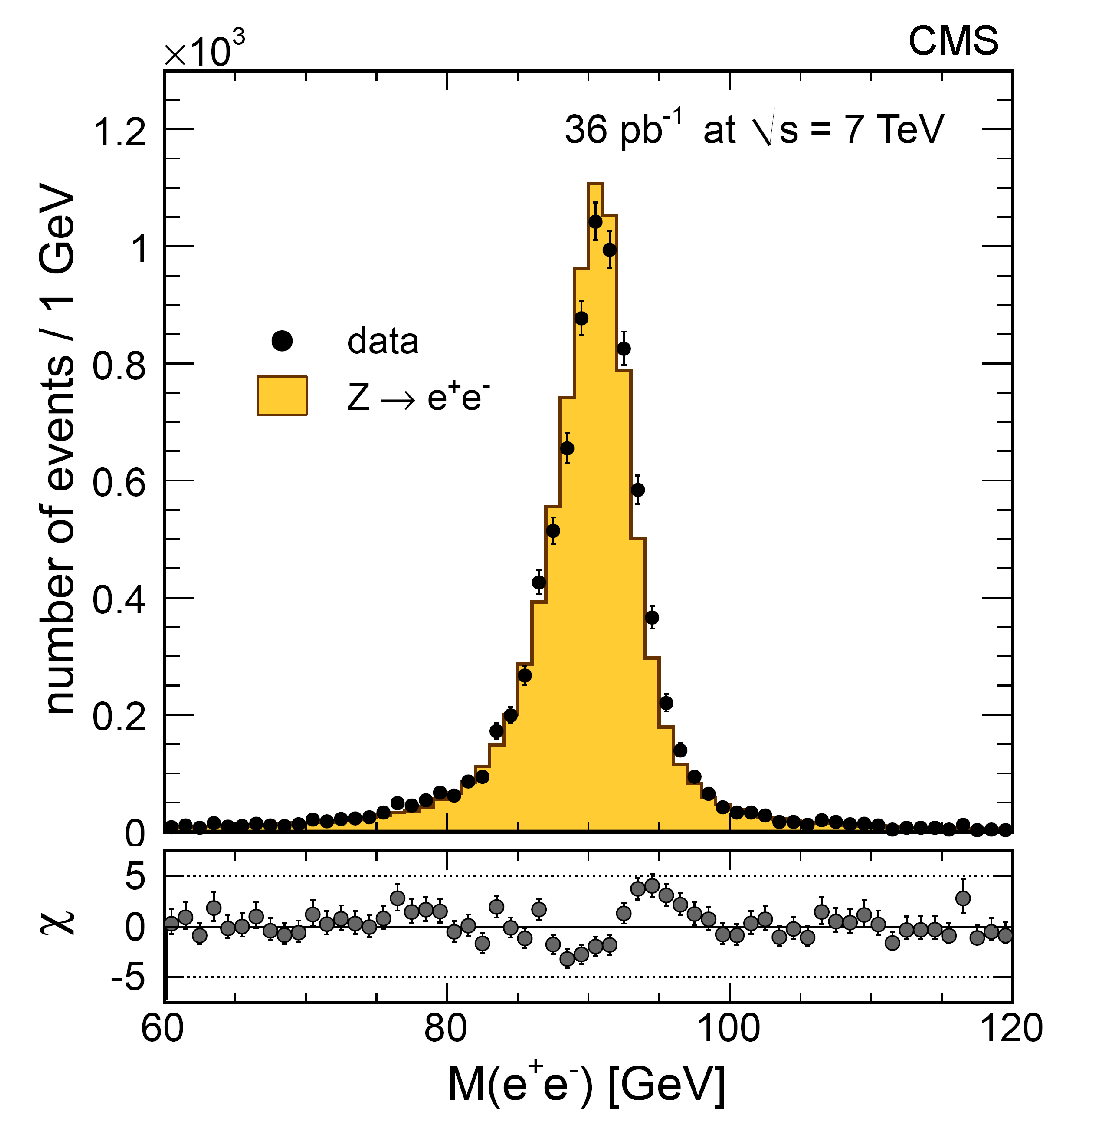
\includegraphics[width=0.48\textwidth]{figs/Zee_mass_Linear.pdf}
   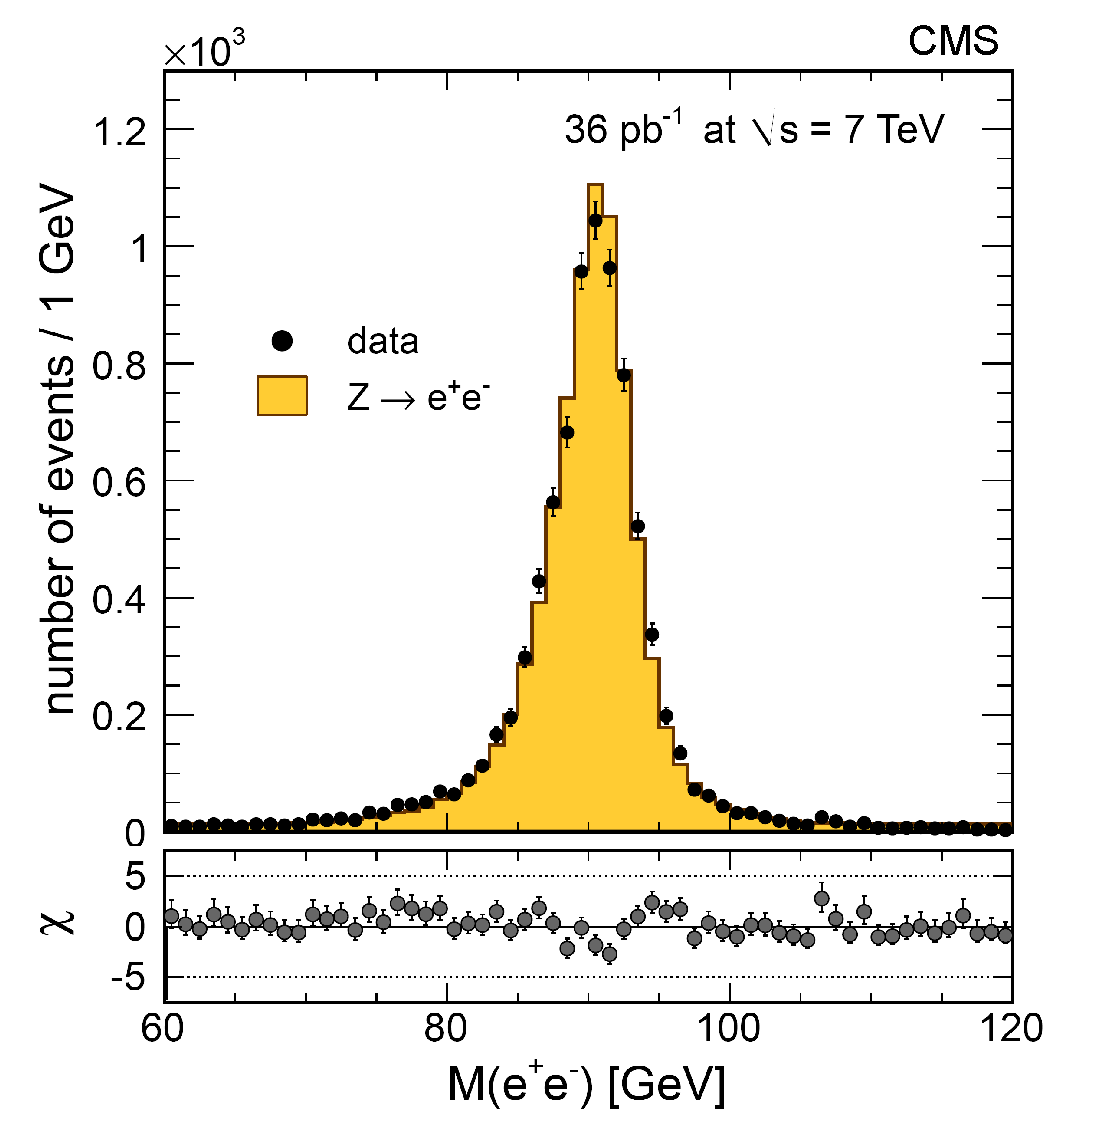
\includegraphics[width=0.48\textwidth]{figs/Zee_mass_Linear_corrected.pdf}
   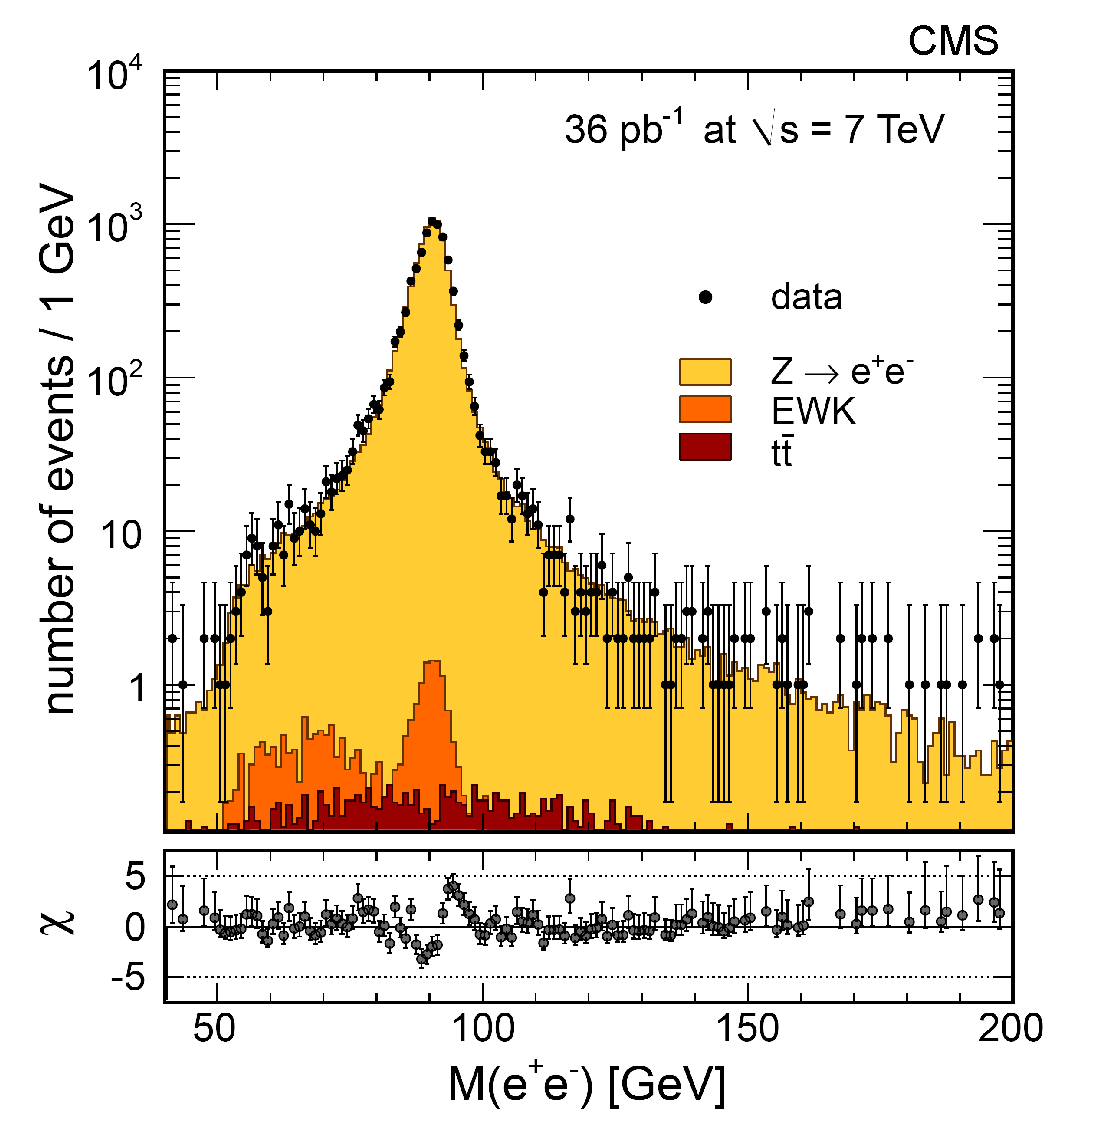
\includegraphics[width=0.48\textwidth]{figs/Zee_mass_Logarithmic.pdf}
   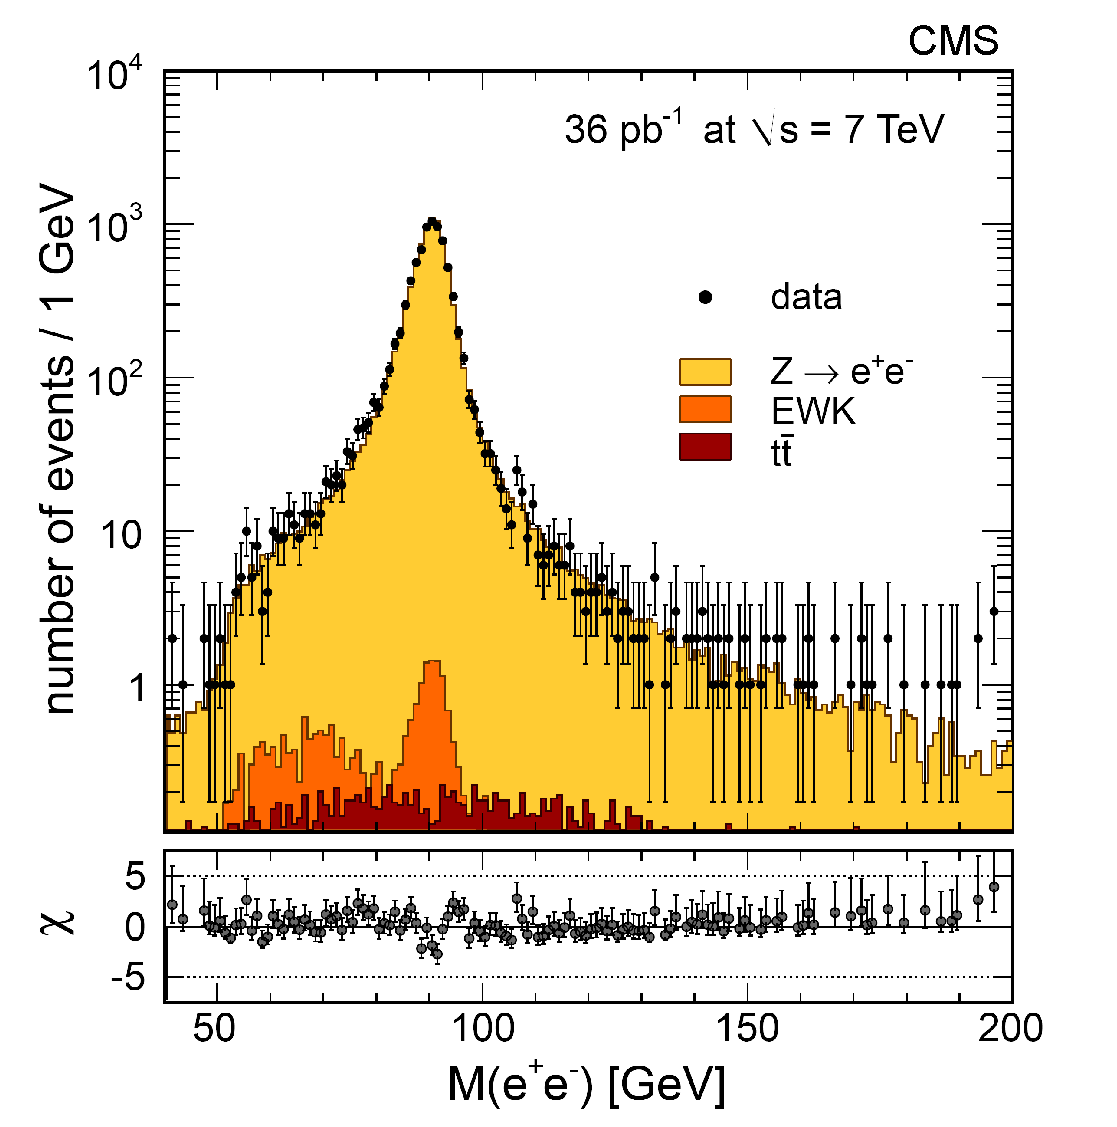
\includegraphics[width=0.48\textwidth]{figs/Zee_mass_Logarithmic_corrected.pdf}
   \caption{ \label{fig:Zee}
Distributions of the dielectron invariant mass for the selected $\Zee$ candidates on
a linear scale (top) and on a logarithmic scale (bottom) before (left)
and after (right) applying energy-scale correction factors.
The points with the error bars represent the data.
Superimposed are the expected distributions from simulations, normalized
to an integrated luminosity of $36$~pb$^{-1}$. The expected distributions are
the Z signal (yellow, light histogram), other EWK processes (orange, medium histogram),
and $\ttbar$ background (red, dark histogram).
Backgrounds are negligible and cannot be seen on the linear-scale plots.
}
  \end{center}
\end{figure}
%%%%%


\subsubsection{Simultaneous Fit}

The $\Zo$ event yield and the electron efficiencies can be extracted from
a simultaneous fit. Two categories of events are
considered: events where both electrons satisfy
the tight selection with $\Et>25\GeV$, and events that consist of
one electron with $\Et>25\GeV$ that passes the tight selection, and one
ECAL cluster with $\Et>25\GeV$ that fails
the selection, either at the reconstruction or electron identification level.

In each category, a signal-plus-background function is fitted to the observed mass spectrum.
The signal shape is taken from signal samples simulated with POWHEG at the NLO generator level,
and is convolved with a Crystal-Ball function modified to include an extra
Gaussian on the high end tail with floating mean and width.
In the first category, the nearly vanishing background is fixed to the
value reported in Table~\ref{tab:ZllBG}. In the second
category of events, the background is modeled by an exponential distribution.

Assuming that $N_\mathrm{signal}^\mathrm{pass}$ is the number of signal events of the first 
category and $N_\mathrm{signal}^\mathrm{fail}$ is the number of the signal events of the 
second category, then:
\begin{eqnarray}
 \label{eqSIMFIT_Pass}
   N_\mathrm{signal}^\mathrm{pass} & = & N^0_\mathrm{ee}\epsilon_\mathrm{rec,tight}^2[1 - (1 - \EPS{\tnp-trg})^2]\,,  \\
  \label{eqSIMFIT_Fail}
   N_\mathrm{signal}^\mathrm{fail} & = & 2N^0_\mathrm{ee}\epsilon_\mathrm{rec,tight}(1 - \epsilon_\mathrm{rec,tight})\EPS{\tnp-trg}\,,  \\
% \label{eqSIMFIT_Nee}
%   N_^0\mathrm{ee} & = & \sigma\mathrm{(pp \rightarrow ZX)}\times{\cal B}\mathrm{(Z \rightarrow e^+e^-)}~{\cal L}~A_\mathrm{Z}\mathrm{(e)}  
%   N_\mathrm{ee}^0 & = & \sigma_\mathrm{Z \rightarrow e^+e^-}~{\cal L}~A_\mathrm{Z}\mathrm{(e)}  
\end{eqnarray}
where $N^0_\mathrm{ee}$ is the number of the expected signal events within the acceptance $A_\mathrm{Z}\mathrm{(e)}$ defined in
Section~\ref{sec:acceptance},
% $\sigma_\mathrm{Z \rightarrow e^+e^-}$ is the measured cross section, ${\cal L}$ is the integrated 
% luminosity, 
$\epsilon_\mathrm{rec,tight}$~=~$\epsilon_\mathrm{rec}$$\epsilon_\mathrm{tight}$ is the measured product of efficiencies
as they are defined in Section~\ref{sec:ELEefficiencies}, and $\EPS{\tnp-trg}$ are the values reported in Table~\ref{tab:e-eff-summary}.

%Fig.~\ref{fig:Zmass_TT_TF} shows the fit to the Tag-Tag events (left plot) and to
%Tag-Fail events (right plot).
The estimated cross section is $988 \pm 10\, \mathrm{(stat.)} \pm 4\mathrm{(syst.)}\,\mathrm{pb}$.
The cross section is in good agreement with the counting analysis estimate of
 $992 \pm 11\, \mathrm{(stat.)}\,\mathrm{pb}$, considering only the statistical uncertainty.
Both techniques give equivalent results. The counting analysis estimate is used for the
cross section measurement in the $\Zee$ channel.

%\begin{figure}
%  \begin{center}
%   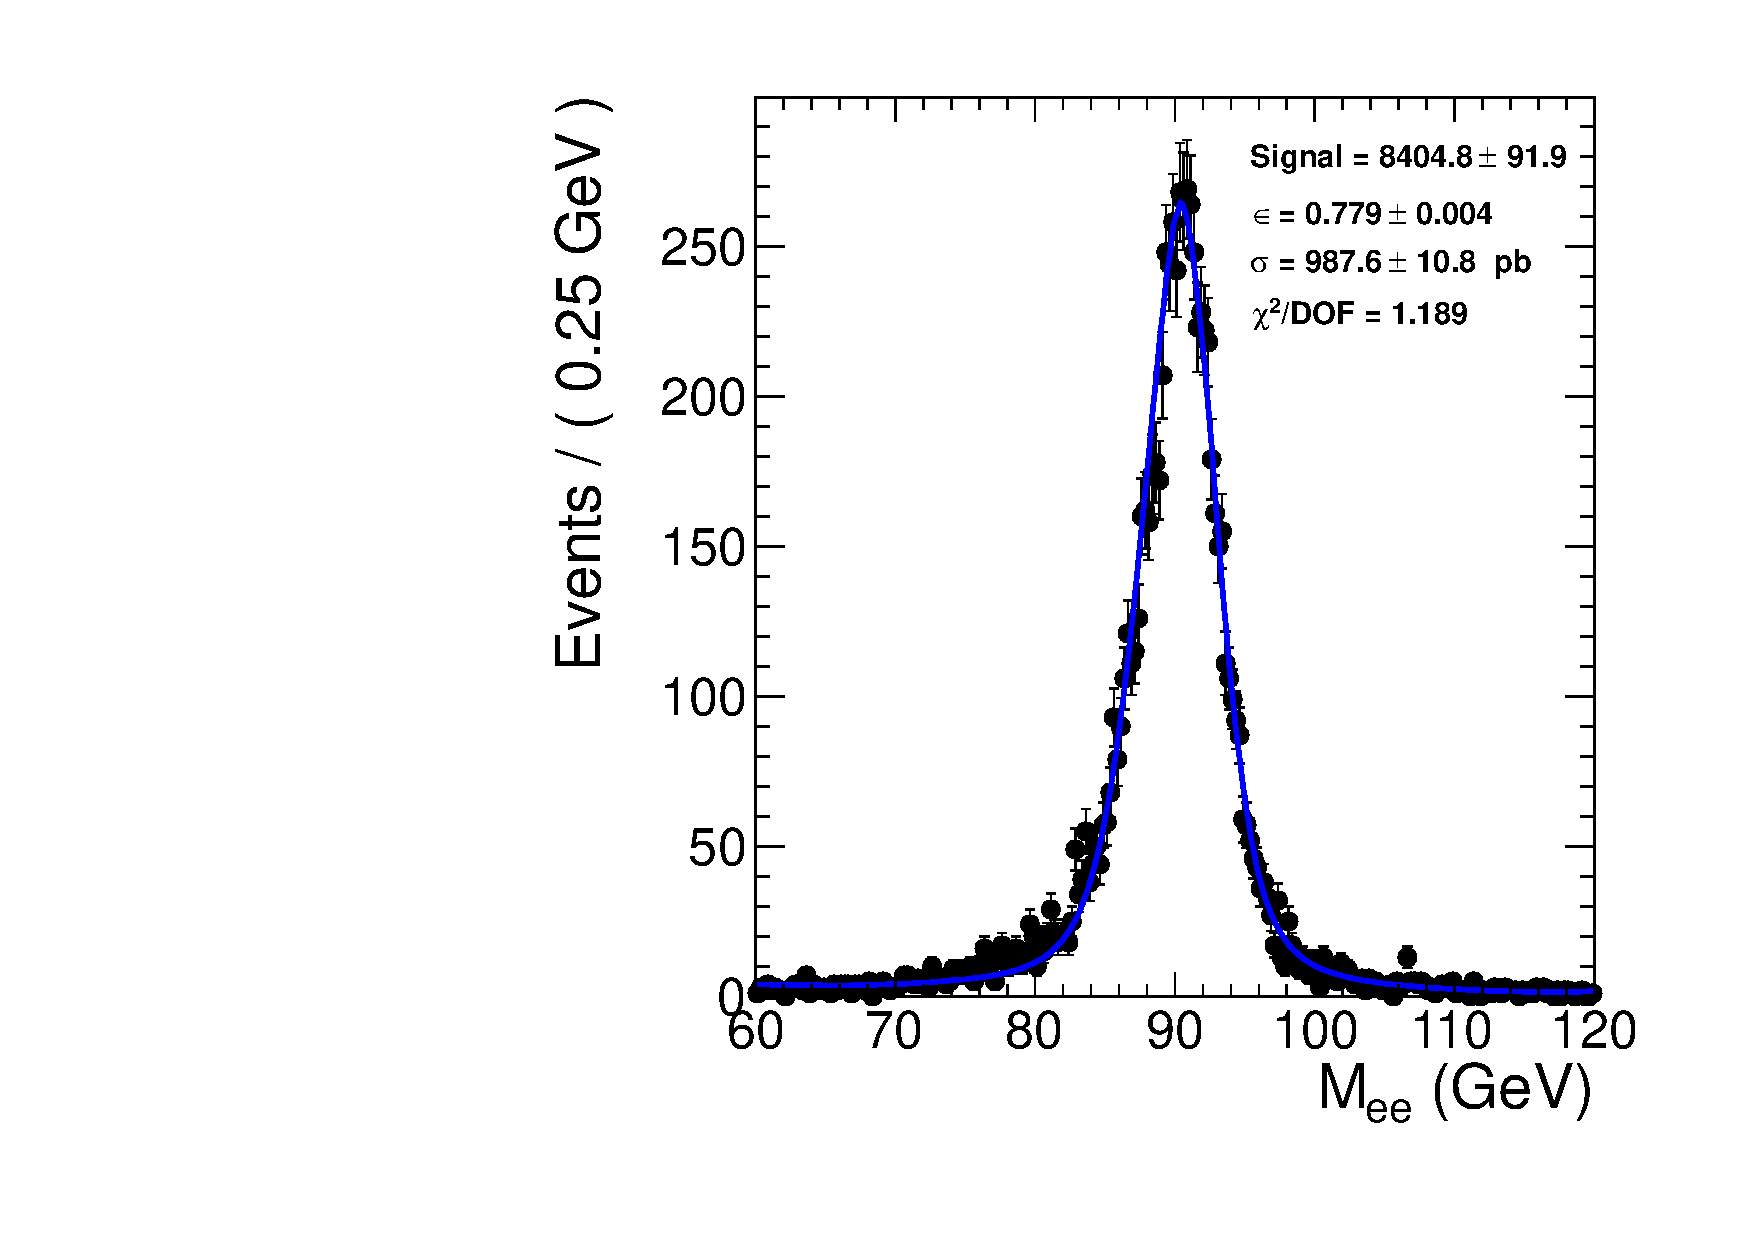
\includegraphics[width=0.48\textwidth]{figs/Zmass_TT_36143nb.pdf}
%   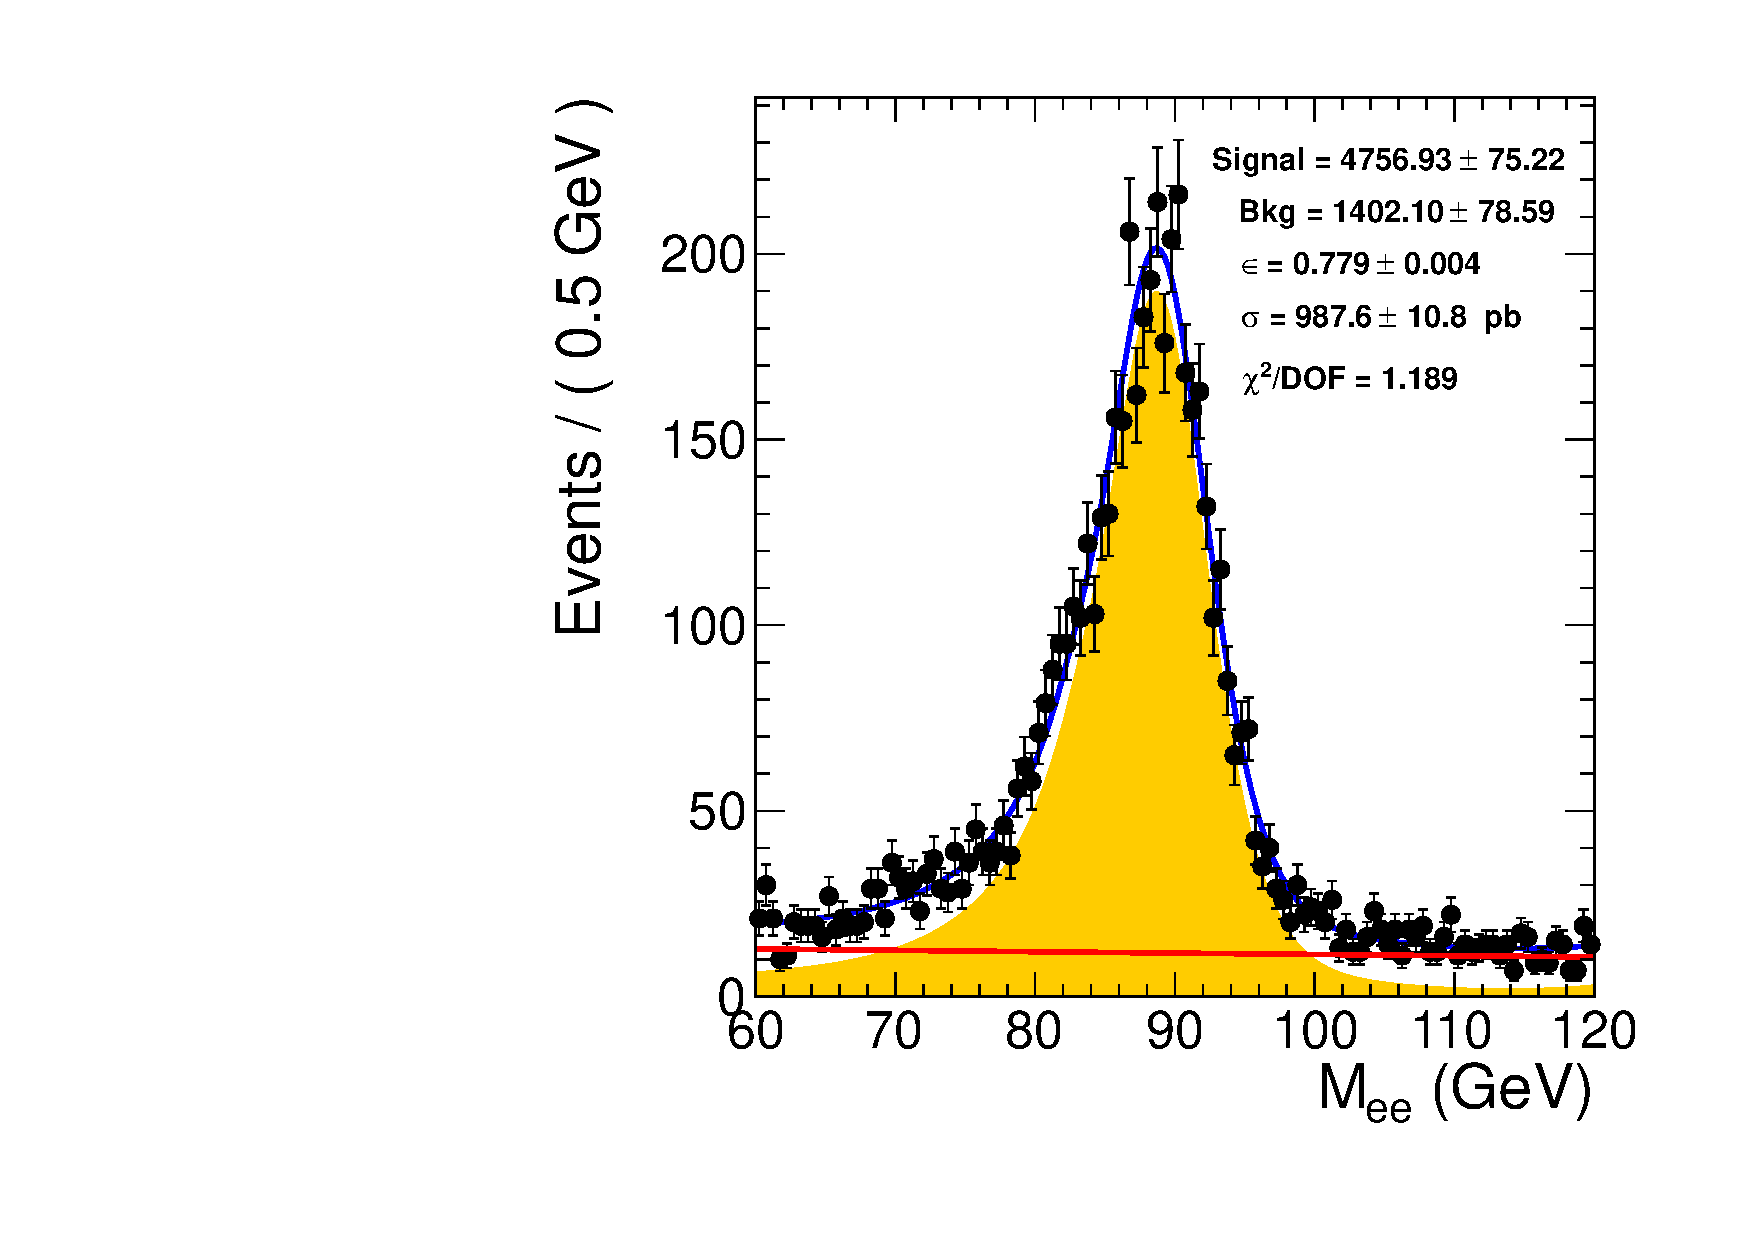
\includegraphics[width=0.48\textwidth]{figs/Zmass_TF_36143nb.pdf}
%   \caption{ \label{fig:Zmass_TT_TF}
%Fits to the Tag-Tag mass distributions (left plot) and Tag-Fail mass distributions (right plot)
%used in the simultaneous determination of the Zee yield and the electron efficiencies. }
%  \end{center}
%\end{figure}

%The electron $p_T$ distribution for $\Zee$ is shown in
%Fig.~\ref{fig:ZpT} in Appendix~\ref{sec:KinDist}.  Also,
%Fig.~\ref{fig:Zkin} shows the dielectron transverse
%momentum ($q_T$) and rapidity ($Y$) distributions.

